\documentclass[conference,10pt]{IEEEtran}

\usepackage[utf8]{inputenc}
\usepackage[T1]{fontenc}
\usepackage{graphicx}
\usepackage{float}
\usepackage{amsmath,amssymb}
\usepackage{booktabs}
\usepackage{array}
\usepackage{hyperref}
\usepackage{cite}

\hypersetup{
    colorlinks=true,
    linkcolor=black,
    urlcolor=blue,
    citecolor=black
}

\graphicspath{{diagram/}}

\renewcommand{\figurename}{Gbr.}
\renewcommand{\tablename}{Tabel}

\newcolumntype{L}[1]{>{\raggedright\let\newline\\\arraybackslash\hspace{0pt}}m{#1}}
\newcolumntype{C}[1]{>{\centering\let\newline\\\arraybackslash\hspace{0pt}}m{#1}}
\newcolumntype{R}[1]{>{\raggedleft\let\newline\\\arraybackslash\hspace{0pt}}m{#1}}

\begin{document}

\title{Analisis dan Perancangan Use Case Diagram\\Sistem Mesin ATM}

\author{\IEEEauthorblockN{Fatih Jawwad Al Mumtaz}
\IEEEauthorblockA{Program Studi Teknik Informatika\\
Fakultas Sains dan Teknologi\\
Universitas Darussalam Gontor\\
Email: 452024611047@mhs.unida.gontor.ac.id}}

\maketitle

\begin{abstract}
Laporan ini menyajikan analisis dan perancangan use case diagram untuk sistem mesin ATM berdasarkan studi kasus yang diberikan. Mesin ATM beroperasi 24 jam dengan layanan penarikan tunai dan informasi saldo. Sistem melakukan verifikasi PIN dengan batas maksimal tiga kali percobaan. Analisis mencakup identifikasi aktor, skenario, dan relasi antar use case. Diagram use case dirancang menggunakan PlantUML.
\end{abstract}

\section{Pendahuluan}

Mesin ATM (Anjungan Tunai Mandiri) merupakan salah satu sistem yang paling sering digunakan dalam kehidupan sehari-hari. Sistem ini memungkinkan nasabah melakukan transaksi perbankan secara mandiri tanpa bantuan teller. Studi kasus ini menganalisis sistem ATM dengan ketentuan sebagai berikut:

\begin{enumerate}
\item ATM beroperasi 24 jam sehari.
\item Transaksi yang dilayani: penarikan tunai dan informasi saldo.
\item Verifikasi keamanan menggunakan kode PIN.
\item Jika salah PIN sebanyak 3 kali, kartu ditelan mesin.
\item Uang tunai diisi ulang rutin 2 hari sekali atau insidental jika habis sebelum waktunya.
\end{enumerate}

\section{Identifikasi Aktor}

Berdasarkan analisis studi kasus, terdapat dua aktor yang berinteraksi dengan sistem:

\begin{enumerate}
\item \textbf{Nasabah} --- Aktor utama yang menggunakan layanan ATM untuk melakukan transaksi penarikan tunai dan pengecekan saldo. Nasabah harus melalui proses verifikasi PIN sebelum dapat mengakses layanan.
\item \textbf{Petugas} --- Aktor pendukung yang bertanggung jawab mengisi ulang uang tunai dalam mesin ATM. Pengisian dilakukan rutin setiap 2 hari sekali, atau secara insidental jika stok uang tunai habis sebelum waktunya.
\end{enumerate}

\section{Use Case Diagram}

Gambar \ref{fig:usecase} menunjukkan use case diagram sistem ATM yang dirancang.

\begin{figure}[H]
\centering
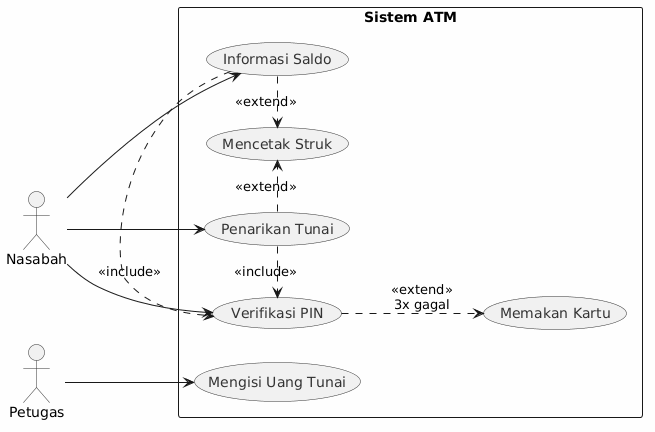
\includegraphics[width=0.95\columnwidth]{usecase.png}
\caption{Use Case Diagram Sistem ATM}
\label{fig:usecase}
\end{figure}

\section{Deskripsi Use Case}

\subsection{Verifikasi PIN}

\begin{center}
\begin{tabular}{|L{2.3cm}|L{5cm}|}
\hline
\textbf{Use Case} & Verifikasi PIN \\
\hline
\textbf{Aktor} & Nasabah \\
\hline
\textbf{Deskripsi} & Nasabah memasukkan kartu ATM dan mengetikkan PIN untuk memverifikasi identitas sebelum melakukan transaksi. \\
\hline
\textbf{Prekondisi} & Kartu ATM dimasukkan dan terbaca sistem. \\
\hline
\textbf{Postkondisi} & Nasabah terverifikasi dan dapat mengakses menu transaksi, atau kartu ditelan jika 3 kali gagal. \\
\hline
\textbf{Skenario Normal} &
\begin{enumerate}
\setlength\itemsep{0pt}
\item Nasabah memasukkan kartu ATM.
\item Sistem meminta PIN.
\item Nasabah memasukkan PIN.
\item Sistem memverifikasi PIN.
\item PIN benar, sistem menampilkan menu transaksi.
\end{enumerate} \\
\hline
\textbf{Skenario Alternatif} &
4a. PIN salah.
\begin{enumerate}
\setlength\itemsep{0pt}
\item[4a1.] Sistem menampilkan pesan error dan sisa percobaan.
\item[4a2.] Kembali ke langkah 2.
\end{enumerate} \\
\hline
\textbf{Skenario Error} &
4b. PIN salah 3 kali berturut-turut.
\begin{enumerate}
\setlength\itemsep{0pt}
\item[4b1.] Sistem menampilkan pesan bahwa kartu akan ditelan.
\item[4b2.] Sistem memanggil use case Memakan Kartu.
\end{enumerate} \\
\hline
\end{tabular}
\end{center}

\subsection{Penarikan Tunai}

\begin{center}
\begin{tabular}{|L{2.3cm}|L{5cm}|}
\hline
\textbf{Use Case} & Penarikan Tunai \\
\hline
\textbf{Aktor} & Nasabah \\
\hline
\textbf{Deskripsi} & Nasabah menarik sejumlah uang tunai dari mesin ATM. \\
\hline
\textbf{Prekondisi} & Nasabah telah terverifikasi melalui use case Verifikasi PIN. \\
\hline
\textbf{Postkondisi} & Uang tunai dikeluarkan, saldo berkurang, dan struk opsional dicetak. \\
\hline
\textbf{Skenario Normal} &
\begin{enumerate}
\setlength\itemsep{0pt}
\item Nasabah memilih menu penarikan tunai.
\item Sistem menampilkan pilihan nominal atau input jumlah.
\item Nasabah memilih atau memasukkan jumlah.
\item Sistem memeriksa ketersediaan saldo dan stok uang.
\item Sistem mengeluarkan uang.
\item Sistem memperbarui saldo.
\item Sistem menawarkan cetak struk.
\end{enumerate} \\
\hline
\textbf{Skenario Alternatif} &
5a. Saldo tidak mencukupi.
\begin{enumerate}
\setlength\itemsep{0pt}
\item[5a1.] Sistem menampilkan pesan saldo tidak cukup.
\item[5a2.] Kembali ke langkah 2.
\end{enumerate}
5b. Stok uang tunai habis.
\begin{enumerate}
\setlength\itemsep{0pt}
\item[5b1.] Sistem menampilkan pesan mesin tidak memiliki cukup uang.
\item[5b2.] Kembali ke menu utama.
\end{enumerate} \\
\hline
\end{tabular}
\end{center}

\subsection{Informasi Saldo}

\begin{center}
\begin{tabular}{|L{2.3cm}|L{5cm}|}
\hline
\textbf{Use Case} & Informasi Saldo \\
\hline
\textbf{Aktor} & Nasabah \\
\hline
\textbf{Deskripsi} & Nasabah mengecek saldo rekening terkini. \\
\hline
\textbf{Prekondisi} & Nasabah telah terverifikasi melalui use case Verifikasi PIN. \\
\hline
\textbf{Postkondisi} & Saldo ditampilkan di layar, dan struk opsional dicetak. \\
\hline
\textbf{Skenario Normal} &
\begin{enumerate}
\setlength\itemsep{0pt}
\item Nasabah memilih menu informasi saldo.
\item Sistem menampilkan saldo rekening.
\item Sistem menawarkan cetak struk.
\end{enumerate} \\
\hline
\end{tabular}
\end{center}

\subsection{Mencetak Struk}

\begin{center}
\begin{tabular}{|L{2.3cm}|L{5cm}|}
\hline
\textbf{Use Case} & Mencetak Struk \\
\hline
\textbf{Aktor} & Nasabah \\
\hline
\textbf{Deskripsi} & Nasabah memilih untuk mencetak struk sebagai bukti transaksi. \\
\hline
\textbf{Prekondisi} & Nasabah selesai melakukan transaksi dan memilih opsi cetak struk. \\
\hline
\textbf{Postkondisi} & Struk berisi detail transaksi tercetak. \\
\hline
\textbf{Skenario Normal} &
\begin{enumerate}
\setlength\itemsep{0pt}
\item Nasabah memilih opsi cetak struk.
\item Sistem mencetak struk berisi detail transaksi.
\item Nasabah mengambil struk.
\end{enumerate} \\
\hline
\textbf{Skenario Alternatif} &
2a. Kertas struk habis.
\begin{enumerate}
\setlength\itemsep{0pt}
\item[2a1.] Sistem menampilkan pesan struk tidak dapat dicetak.
\item[2a2.] Transaksi tetap selesai tanpa struk.
\end{enumerate} \\
\hline
\end{tabular}
\end{center}

\subsection{Memakan Kartu}

\begin{center}
\begin{tabular}{|L{2.3cm}|L{5cm}|}
\hline
\textbf{Use Case} & Memakan Kartu \\
\hline
\textbf{Aktor} & Sistem (otomatis) \\
\hline
\textbf{Deskripsi} & Sistem menelan kartu ATM setelah nasabah gagal memasukkan PIN sebanyak 3 kali. \\
\hline
\textbf{Prekondisi} & Nasabah telah gagal memasukkan PIN 3 kali berturut-turut. \\
\hline
\textbf{Postkondisi} & Kartu ATM ditahan oleh mesin, sesi berakhir. \\
\hline
\textbf{Skenario Normal} &
\begin{enumerate}
\setlength\itemsep{0pt}
\item Sistem menampilkan pesan bahwa kartu ditahan.
\item Sistem menelan kartu.
\item Sesi berakhir.
\end{enumerate} \\
\hline
\end{tabular}
\end{center}

\subsection{Mengisi Uang Tunai}

\begin{center}
\begin{tabular}{|L{2.3cm}|L{5cm}|}
\hline
\textbf{Use Case} & Mengisi Uang Tunai \\
\hline
\textbf{Aktor} & Petugas \\
\hline
\textbf{Deskripsi} & Petugas mengisi ulang uang tunai ke dalam mesin ATM secara rutin (2 hari sekali) atau insidental jika stok habis sebelum waktunya. \\
\hline
\textbf{Prekondisi} & Petugas memiliki akses ke panel mesin ATM. \\
\hline
\textbf{Postkondisi} & Stok uang tunai dalam mesin bertambah sesuai jumlah yang diisi. \\
\hline
\textbf{Skenario Normal} &
\begin{enumerate}
\setlength\itemsep{0pt}
\item Petugas membuka panel mesin ATM.
\item Petugas memasukkan uang tunai ke dalam cassette.
\item Sistem mencatat jumlah uang yang diisi.
\item Petugas menutup panel mesin.
\end{enumerate} \\
\hline
\textbf{Skenario Alternatif} &
3a. Jumlah uang melebihi kapasitas maksimal.
\begin{enumerate}
\setlength\itemsep{0pt}
\item[3a1.] Sistem menampilkan peringatan.
\item[3a2.] Petugas mengurangi jumlah uang.
\item[3a3.] Kembali ke langkah 3.
\end{enumerate} \\
\hline
\end{tabular}
\end{center}

\section{Relasi Antar Use Case}

Tabel \ref{tbl:relasi} merangkum relasi antar use case dalam sistem.

\begin{table}[H]
\centering
\caption{Relasi Antar Use Case}
\label{tbl:relasi}
\begin{tabular}{|l|l|l|}
\hline
\textbf{Use Case} & \textbf{Relasi} & \textbf{Use Case Terkait} \\
\hline
Penarikan Tunai & \texttt{<<include>>} & Verifikasi PIN \\
Informasi Saldo & \texttt{<<include>>} & Verifikasi PIN \\
Verifikasi PIN & \texttt{<<extend>>} & Memakan Kartu \\
Penarikan Tunai & \texttt{<<extend>>} & Mencetak Struk \\
Informasi Saldo & \texttt{<<extend>>} & Mencetak Struk \\
\hline
\end{tabular}
\end{table}

\section{Kesimpulan}

Berdasarkan analisis studi kasus mesin ATM, diidentifikasi dua aktor yaitu Nasabah dan Petugas, serta enam use case: Verifikasi PIN, Penarikan Tunai, Informasi Saldo, Mencetak Struk, Memakan Kartu, dan Mengisi Uang Tunai. Relasi \texttt{<<include>>} digunakan untuk menunjukkan bahwa Penarikan Tunai dan Informasi Saldo memerlukan Verifikasi PIN. Relasi \texttt{<<extend>>} digunakan untuk kondisi opsional seperti Mencetak Struk dan skenario error seperti Memakan Kartu akibat 3 kali gagal PIN. Diagram use case yang dihasilkan memberikan gambaran fungsionalitas sistem secara jelas dan sesuai dengan kebutuhan yang telah ditentukan.

\end{document}
